\subsection{Extensions: Sirius's criterion moved over the study}\label{sec:ext}
Model~D gives every session its own bias, but it treats the sessions as interchangeable: it expects no order in them.
There is order (Fig.~\ref{fig:time}).
Sirius's unimanual PSE rose over the study, most clearly for the right hand: it called fewer unimanual targets ``high'' in the later sessions, which were also the sessions with the strongest distractors.

Two extensions describe this with one extra parameter per hand.
In \textbf{D+crit} the session bias follows the session's distractor amplitude; in \textbf{D+order} it drifts linearly with the session's place in the study.
\begin{itemize}
\item Both predict clearly better than D, above all for new sessions: D+crit by \CritvsDTrial\ $\pm$ \CritvsDTrialSE\ at the trial level and \CritvsDLoso\ $\pm$ \CritvsDLosoSE\ for new sessions (better on \CritvsDLosoNbetter\ of 42), D+order by \OrdervsDTrial\ $\pm$ \OrdervsDTrialSE\ and \OrdervsDLoso\ $\pm$ \OrdervsDLosoSE.
No other single addition to D comes close; the next best, a shared daily bias, gains \SharedvsDLoso\ for new sessions.
\item The two cannot be told apart. D+crit minus D+order is \CritvsOrderTrial\ $\pm$ \CritvsOrderTrialSE\ at the trial level and \CritvsOrderLoso\ $\pm$ \CritvsOrderLosoSE\ for new sessions. A model with both terms is no better than either (\CritOrdervsCritLoso\ $\pm$ \CritOrdervsCritLosoSE\ over D+crit), and in it neither coefficient is clearly different from zero.
The design does not allow the distinction: the distractor amplitude was raised steadily, so it is correlated 0.91 with the session order. Only the four 24\um\ sessions run late in the study break the pattern, and they do not settle it: three lean slightly towards drift and one towards adaptation (together $-1.5$ elpd for D+crit against D+order).
\item The size of the change: in a typical session the unimanual PSE is \critPseLeft\um\ higher in the 32\um\ sessions than in the 6\um\ sessions for the left hand (95\% interval \critPseLeftLo\ to \critPseLeftHi) and \critPseRight\um\ higher for the right (\critPseRightLo\ to \critPseRightHi), comparable to the bimanual shift itself.
For the left hand the rise roughly offsets the distractor's push: the overall proportion of ``high'' answers to left-hand targets stays between 0.44 and 0.49 in every amplitude group, while unimanual ``high'' answers fall from 0.44 to 0.39 and bimanual ones rise from 0.45 to 0.54. For the right hand the criterion rose further than that.
\end{itemize}

Modelling the trend changes one conclusion of the previous report.
When every session's bias is pulled toward a single value (Model~D), part of the trend is absorbed by the bimanual terms, because the bias is shared by a session's unimanual and bimanual trials.
With the trend modelled, the bimanual shift grows more steeply with amplitude ($b_2=\muBtwoCritLeft$ left and \muBtwoCritRight\ right, against \muBtwoDLeft\ and \muBtwoDRight\ in D) and the presence offset shrinks.
For the right hand it remains clear ($b_3=\muBthreeCritRight$, \muBthreeCritRightLo\ to \muBthreeCritRightHi); for the left hand it is no longer distinguishable from zero (\muBthreeCritLeft, \muBthreeCritLeftLo\ to \muBthreeCritLeftHi).
The shift averaged over sessions, the JND result and the lapse pattern do not change (Table~\ref{tab:effects}).

\paragraph{A shared daily bias}
The two hands' session biases are correlated (0.50 between their unimanual PSEs in Model~D, 0.36 to 0.41 after a linear trend in amplitude or time is removed). A daily offset shared by the hands (D+shared) improves on D (\SharedvsDTrial\ $\pm$ \SharedvsDTrialSE\ at the trial level, \SharedvsDLoso\ $\pm$ \SharedvsDLosoSE\ for new sessions), but much less than the trend does for new sessions (D+shared minus D+crit: \SharedvsCritLoso\ $\pm$ \SharedvsCritLosoSE): much of what the hands share from day to day is the trend. Added to E, the shared offset is small ($\sigma_v=\sigSharedEshared$ on the logit scale) and gains little (\EsharedvsETrial\ $\pm$ \EsharedvsETrialSE\ at the trial level, \EsharedvsELoso\ $\pm$ \EsharedvsELosoSE\ for new sessions).

\begin{figure}[tbp]
\centering
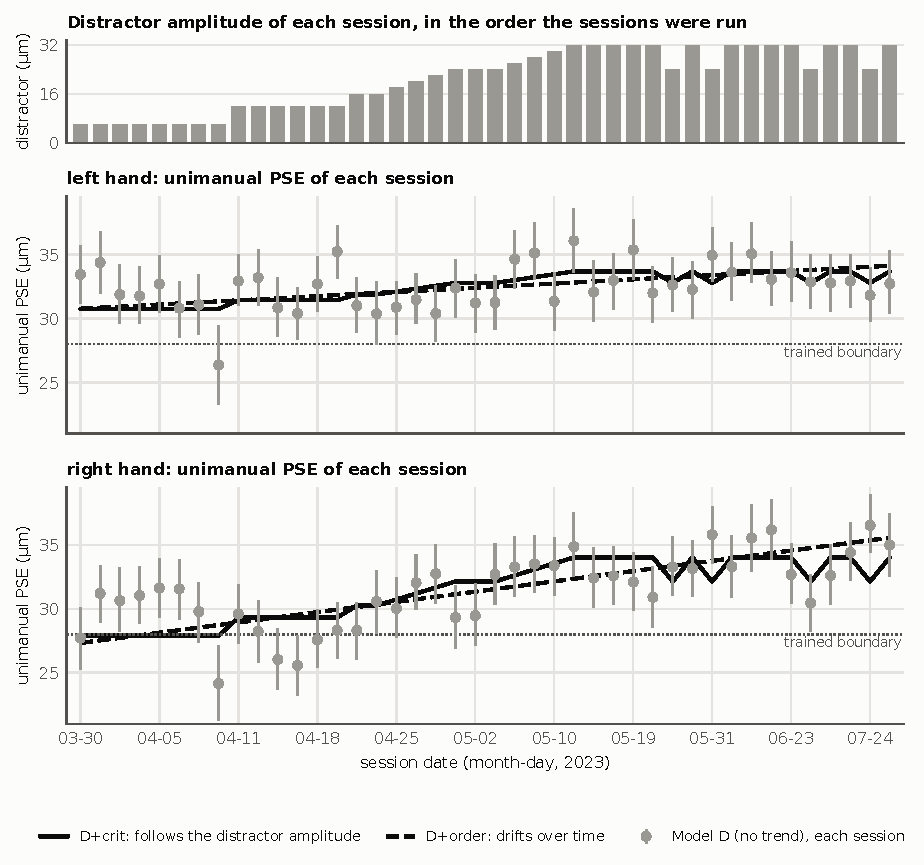
\includegraphics[width=\textwidth]{../results5000/figs/F6_bias_time_amplitude.pdf}
\caption{Top: the distractor amplitude of each session, in the order the sessions were run.
Middle and bottom: each session's unimanual PSE in Model~D, which assumes no trend (grey, 95\% intervals), with the typical-session PSE of the two extensions:
the bias follows the distractor amplitude (D+crit, solid) or drifts linearly over time (D+order, dashed).
Both lines track the rise; only the four late 24\um\ sessions could separate them.}\label{fig:time}
\end{figure}
